\begin{figure}[H]
    \centering
    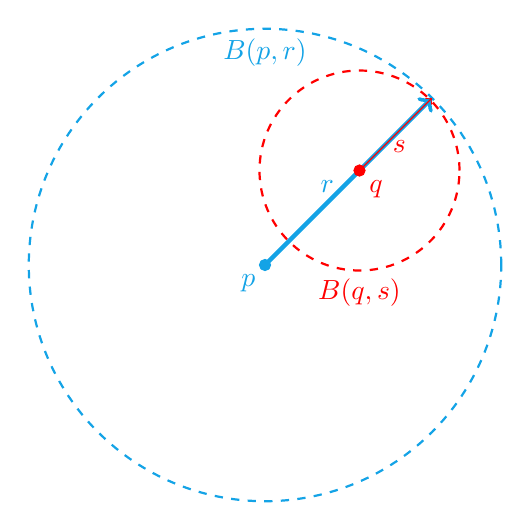
\begin{tikzpicture}
    % Bola B(p, r)
    \draw[thick, dashed, Cerulean] (0,0) circle (3);
    \filldraw[Cerulean] (0,0) circle (2pt) node[below left] {$p$};
    \node[Cerulean] at (0,2.7) {$B(p, r)$};
    % Raio r
    \draw[ultra thick,Cerulean,->] (0,0) -- (2.12,2.12);
    \node[Cerulean, left] at (1,1) {$r$};

    % Bola B(q, s)
    \filldraw[Red] (1.2,1.2) circle (2pt) node[below right] {$q$};
    \draw[thick, dashed, Red] (1.2,1.2) circle (1.27);
    \node[Red] at (1.2,-0.35) {$B(q, s)$};
    % Raio s
    \draw[Red,->] (1.2,1.2) -- (2.12,2.12);
    \node[Red, right] at (1.5,1.5) {$s$};

    % Relação de inclusão
    \end{tikzpicture}
    \caption{Relação de inclusão entre as bolas abertas.}
    \label{fig:abertosBolaAberta}
\end{figure}
